\documentclass{bmstu}

\usepackage[fontsize=14pt]{fontsize}

\bibliography{biblio}

\begin{document}

\makecourseworktitle
    {Информатика, искусственный интеллект и системы управления} % Название факультета
    {Программное обеспечение ЭВМ и информационные технологии} % Название кафедры
    {Протокол бессерверных конференций} % Тема работы
    {Клименко~А.~К./ИУ7-31М} % Номер группы/ФИО студента (если авторов несколько, их необходимо разделить запятой)
    {Никульшин~А.~М.} % ФИО научного руководителя
    {} % ФИО консультанта (необязательный аргумент; если консультантов несколько, их необходимо разделить запятой)

\setcounter{page}{3}

{\fontsize{12pt}{1em}
\selectfont
\maketableofcontents

%\begin{definitions}
	\definition{}{}
\end{definitions}
%\include{02-abbreviations}

\chapter*{ВВЕДЕНИЕ}
\addcontentsline{toc}{chapter}{ВВЕДЕНИЕ}

Целью данной работы является проектирование протокола проведения бессерверных аудио видео конференций.
Для достижения поставленной цели необходимо решить следующие задачи:
\begin{itemize}[label=---]
    \item изучить схожие протоколы;
    \item спроектировать протокол бессерверных конференций;
    \item реализовать ПО осуществляющее взаимодействие по разработанному протоколу;
    \item протестировать ПО.
\end{itemize}

\chapter{Аналитический раздел}

\section{Актуальность}

Одной из наиболее актуальных задач в современном мире является обеспечение эффективного взаимодействия между удаленными пользователями.
Бессерверные аудио-видео конференции представляют собой перспективное решение, позволяющее организовывать виртуальные встречи без необходимости использования централизованных серверов.

Традиционные подходы к организации конференц-связи, основанные на клиент-серверной архитектуре, сталкиваются с рядом ограничений.
Во-первых, они требуют наличия мощной серверной инфраструктуры, которая должна обрабатывать весь трафик участников, что приводит к высоким эксплуатационным расходам.
Во-вторых, централизованные системы являются уязвимыми к сбоям и атакам, так как отказ сервера может привести к полной потере связи между пользователями.
В-третьих, такие решения зачастую ограничены в масштабируемости, что затрудняет их применение в крупномасштабных распределенных средах.

Бессерверные аудио-видео конференции, в свою очередь, обладают рядом преимуществ.
Они позволяют организовывать виртуальные встречи напрямую между участниками, без необходимости использования централизованных серверов.
Это повышает отказоустойчивость системы, поскольку отказ одного из клиентов не приводит к полной потере связи.
Кроме того, данный подход способствует снижению эксплуатационных расходов и упрощает процесс масштабирования.

Разработка протокола для организации бессерверных аудио-видео конференций является важной научно-технической задачей, имеющей высокую практическую значимость.
Результаты исследования могут найти применение в различных областях, таких как дистанционное обучение, удаленная работа, проведение виртуальных совещаний и конференций, а также во многих других сценариях, требующих эффективного взаимодействия между удаленными участниками.

\section{Потоковая передача данных в реальном времени}

Говоря о аудио-видео конференциях, следует выделить две основные составляющие потоков данных -- аудио поток и видео поток.
Аудио поток, как правило, имеет более высокий приоритет по сравнению с видео потоком, поскольку бесперебойная передача звука является критически важной для обеспечения качественного взаимодействия участников.

Основными протоколами транспортного уровня, используемыми при передаче данных в режиме реального времени, являются TCP, UDP.
На прикладном уровне часто используются такие протоколы как RTP (Real-Time Transport Protocol  \cite{rtp}), RTCP (Real-Time Transport Control Protocol  \cite{rtp}), SIP (Session Initiation Protocol \cite{sip}), H.323 \cite{h323}.

RTP и RTCP обеспечивают передачу аудио и видео с минимальной задержкой, но не предоставляют встроенных механизмов шифрования.
SIP и H.323, напротив, поддерживают управление сессиями и шифрование, но могут быть более сложными в реализации.
На основе этого анализа было принято решение рассмотреть два подхода: TCP+TLS и SRTP, как наиболее подходящие для бессерверных конференций.
Рассмотрим преимущества и недостатки каждого из подходов:

Преимущества использования TCP+TLS:

\begin{itemize}[label=---]
  \item Надежность и безопасность --- TCP гарантирует доставку данных без потерь, а TLS обеспечивает шифрование и аутентификацию, что защищает данные от перехвата и подделки.
  \item Развитая инфраструктура --- TCP и TLS широко поддерживаются, существует множество библиотек и инструментов для их реализации, что упрощает разработку и интеграцию.
\end{itemize}

Недостатки:

\begin{itemize}[label=---]
  \item Более высокая задержка --- TCP имеет больше накладных расходов по сравнению с UDP-протоколами, что может повлиять на качество аудио и видео.
  \item Более высокие требования к ресурсам --- TCP-стек требует больше памяти и вычислительных ресурсов, что может быть критично для устройств с ограниченными возможностями, такими как мобильные устройства или встраиваемые системы.
\end{itemize}

Преимущества использования SRTP:

\begin{itemize}[label=---]
  \item Низкая задержка --- SRTP, построенный поверх UDP, имеет меньше накладных расходов, что позволяет обеспечить более высокое качество аудио и видео.
  \item Меньшее потребление ресурсов --- SRTP более эффективен в плане использования памяти и вычислительной мощности, что важно для мобильных устройств.
  \item Специализация на мультимедиа --- SRTP разработан специально для защищенной передачи аудио и видео данных, в отличие от более универсального TCP+TLS.
\end{itemize}
  
Недостатки: TODO: посмотреть на SRTCP, а не на SRTP

\begin{itemize}[label=---]
  \item Меньшая надежность --- UDP, лежащий в основе SRTP, не гарантирует доставку данных, что может привести к потере пакетов в неблагоприятных сетевых условиях.
  \item Сложность реализации --- SRTP требует реализации дополнительных механизмов для управления ключами шифрования, что усложняет разработку.
\end{itemize}

\section{Распределение вычислений}

При централизованном проведении конференций основная нагрузка ложится на сервер, в то время как при проведении бессерверных конференций она распределяется по клиентам. Для обеспечения наилучшего QoS необходимо учитывать вычислительные возможности каждого клиента, а также пропускную способность каналов, объединяющих их.

В бессерверной архитектуре каждый участник конференции выступает в качестве автономного узла, ответственного за обработку и передачу мультимедийного контента. Это требует от клиентских устройств достаточной вычислительной мощности для кодирования, декодирования и синхронизации аудио, видео и данных в режиме реального времени.

\begin{equation}
  \textit{Perf}_{client} = f(CPU, GPU, RAM)
\end{equation}

Пропускная способность каналов связи также играет критическую роль, определяя максимально возможное качество и разрешение передаваемых потоков. Недостаточная пропускная способность может привести к снижению качества и стабильности соединения, а также к возникновению задержек и потерь пакетов.

\begin{equation}
  \textit{Bandwidth}_{channel}=f(\textit{network~speed},\textit{distance},\textit{noises})
\end{equation}

Для достижения оптимального QoS в бессерверных конференциях необходимо динамически адаптировать параметры кодирования и передачи мультимедийных потоков к возможностям каждого участника. Это может быть реализовано с помощью механизмов согласования характеристик сессии и адаптивного управления скоростью передачи данных.

\section{Микширование}

При большом числе участников в бессерверных видеоконференциях имеет смысл применять микширование передаваемых видео потоков. Это позволяет уменьшить общий объем передаваемых данных, снизив нагрузку на каналы связи, но при этом требует значительных вычислительных ресурсов от клиентских устройств.

Процесс микширования видео можно представить в виде следующих основных шагов:

\begin{enumerate}
\item Получение видео кадров от соседних узлов.
\item Декодирование полученных кадров.
\item Композиция единого кадра путем пространственного объединения (склеивания) исходных кадров.
\item Кодирование скомпонованного кадра.
\item Передача закодированного кадра всем соседним узлам.
\end{enumerate}

При этом, на этапе формирования общего кадра необходимо учитывать, нужен ли тот или иной видео поток каждому из соседних участников. Это позволяет оптимизировать состав композитного кадра и снизить вычислительную нагрузку.

Микширование аудио потоков может быть реализовано схожим образом, с формированием раздельных аудио каналов для каждого участника конференции. Это требует дополнительных вычислений, связанных с микшированием, кодированием и передачей аудио данных.

Эффективность микширования определяется соотношением выигрыша в объеме передаваемых данных и затратами вычислительных ресурсов на клиентских устройствах. Для поддержания высокого качества и низкой задержки передачи мультимедийного контента необходим тщательный подбор алгоритмов микширования и кодирования с учетом возможностей участников конференции.

\section{Устойчивость конференции}

Отключение ключевого участника конференции, через которого проходит большое число потоков данных от других участников, является одной из проблем распределенных вычислений. Решением этой проблемы может послужить механизм, обеспечивающий поддержание <<запасных>> каналов передачи между клиентами.

\section{Защита информации}

Для защиты конференции необходимо использовать защищенные каналы передачи. На каждое соединение инициализируется собственная сессия, вместо того, чтобы использовать одну сессию на всех участников конференции.

Плюсы такого подхода:
\begin{itemize}[label=---]
  \item Повышение безопасности за счет использования индивидуальных криптографических ключей для каждого соединения.
  \item Улучшение масштабируемости системы, так как каждое соединение обрабатывается независимо.
  \item Более гибкое управление доступом и привилегиями участников конференции.
\end{itemize}

Минусы такого подхода:
\begin{itemize}[label=---]
  \item Увеличение вычислительной нагрузки на клиентские устройства, связанное с необходимостью поддержания множества криптографических сессий.
  \item Более высокие требования к пропускной способности канала связи, обусловленные необходимостью передачи дополнительных данных, связанных с криптографической защитой.
\end{itemize}

В программной реализации протокола применяется библиотека OpenSSL \cite{openssl} для осуществления защищенных соединений. Использование OpenSSL позволяет обеспечить совместимость с широким спектром криптографических алгоритмов, а также реализовать такие механизмы безопасности, как аутентификация, шифрование и целостность передаваемых данных. Кроме того, OpenSSL предоставляет средства для управления криптографическими ключами, что упрощает интеграцию защищенных соединений в общую архитектуру системы.

\section{Преодаление NAT}

Одной из ключевых проблем при реализации бессерверных видеоконференций является преодоление ограничений, связанных с трансляцией адресов.
NAT используется для преобразования частных IP-адресов в публичные и наоборот, что позволяет нескольким устройствам в локальной сети использовать один публичный IP-адрес для выхода в интернет.
Однако NAT создает сложности для прямого соединения между участниками, находящимися за разными NAT, так как они не могут напрямую обмениваться данными без дополнительных механизмов.

Для преодоления ограничений NAT в бессерверных конференциях используются следующие подходы:

\begin{enumerate}
  \item STUN (Session Traversal Utilities for NAT).
  STUN --- это протокол, который позволяет участникам, находящимся за NAT, определить свой публичный IP-адрес и порт, назначенный NAT для исходящего соединения.
  Это позволяет участникам обмениваться этой информацией и устанавливать прямое соединение.
  
  Принцип работы STUN заключается в том, что каждый участник отправляет запрос на STUN-сервер, который возвращает ему его публичный IP-адрес и порт.
  Затем они обмениваются этой информацией через сигнальный канал.
  После обмена информацией участники пытаются установить прямое соединение через публичные IP-адреса и порты.
  
  STUN Позволяет установить прямое соединение между участниками, находящимися за NAT.
  Не требует дополнительных серверов для ретрансляции данных.
  Однако, он не работает с симметричным NAT, где порты для входящих и исходящих соединений различаются.
  
  \item TURN (Traversal Using Relays around NAT).
  TURN --- это протокол, который позволяет участникам, находящимся за NAT, использовать ретрансляционный сервер для передачи данных, если прямое соединение невозможно.
  TURN-сервер выступает в качестве посредника, пересылая данные между участниками.
  
  Как работает TURN: участники устанавливают соединение с TURN-сервером и получают от него публичный IP-адрес и порт для ретрансляции данных, после чего обмениваются этой информацией через сигнальный канал.
  Если прямое соединение невозможно, данные передаются через TURN-сервер.
  
  TURN работает с любыми типами NAT, включая симметричный и обеспечивает надежную передачу данных даже в сложных сетевых условиях.
  Но данный подход требует наличия TURN-сервера, что увеличивает затраты на инфраструктуру, а также вводит дополнительную задержку из-за ретрансляции данных через сервер.
  
  \item ICE (Interactive Connectivity Establishment).
  ICE --- это технология, которая объединяет STUN и TURN для установления соединения между участниками.
  ICE автоматически выбирает оптимальный способ соединения: прямое (через STUN) или через ретрансляционный сервер (TURN).
  
  При использовании ICE участники собирают все возможные кандидаты для соединения (локальные IP-адреса, публичные IP-адреса через STUN, ретрансляционные адреса через TURN) и обмениваются списками кандидатов через сигнальный канал.
  ICE проверяет каждый кандидат и выбирает оптимальный путь для соединения.
  
  Преимущества: автоматический выбор лучшего способа соединения, поддержка всех типов NAT, включая симметричный.
  Ограничения: требуются интеграции STUN и TURN серверов, увеличенная сложность реализации.

  \item UPnP (Universal Plug and Play).
  UPnP --- это протокол, позволяющий устройствам автоматически настраивать проброс портов на NAT-устройствах (например, роутерах).
  Если участник поддерживает UPnP, он может автоматически открыть порт для входящих соединений.

  Как работает UPnP: участник отправляет запрос на роутер через UPnP для открытия порта; роутер открывает порт и назначает его для входящих соединений; участник использует этот порт для приема данных от других участников.

  UPnP позволяет участникам принимать входящие соединения без ручной настройки NAT и  упрощает установление прямых соединений.
  Однако не все роутеры его поддерживают, а также он может быть отключен по соображениям безопасности.

  \item Использование P2P-технологий с NAT-пробросом.
  В некоторых случаях можно использовать P2P-технологии, такие как UDP hole punching, которые позволяют участникам устанавливать прямое соединение через NAT без использования промежуточных серверов.

  Участники обмениваются информацией о своих публичных IP-адресах и портах через сигнальный канал, затем одновременно отправляют UDP-пакеты друг другу, что позволяет "пробить" NAT и установить прямое соединение.

  Данный способ не требует дополнительных серверов для ретрансляции данных и подходит для большинства типов NAT, кроме симметричного, однако для его работы требуется точная синхронизация между участниками.
\end{enumerate}

\chapter{Конструкторский раздел}

% \section{Функциональная схема организации конференции}

%На рисунке \ref{img:idef0} представлена функциональная схема организации конференции в нотации IDEF0.

%\includeimage
%    {idef0}
%    {f}
%    {H}
%    {\linewidth}
%    {Функциональная схема организации конференции в нотации IDEF0}

\section{Функциональные требования к протоколу}

Ниже перечислены функциональные требования к разрабатываемому протоколу.

\begin{enumerate}
    \item Протокол должен поддерживать проведение одной конференции для произвольного количества участников.
    \item Участники должны иметь возможность подключаться и отключаться от конференции во время ее проведения.
\end{enumerate}

% \section{Граф переходов состояний для конференции}

% Конференция существует пока в ней есть хотя бы один участник.

% Конференция может находиться в следующих состояниях:

% \begin{enumerate}
%     \item Удалена или еще не создана.
%     \item Подготовительное.
%     \item Активное.
% \end{enumerate}

% В подготовительном состоянии происходит определение ролей всех участников, а также подготовка каналов передачи данных. При отключении одного из участников или подключении нового участника конференция также переходит в данное состояние.

\section{Роли участников конференции}

При создании конференции участник, который ее создает (и отправляет приглашения остальным участникам) назначается управляющим конференцией.

Управляющий конференцией имеет возможность редактировать параметры конференции, рассылать приглашения, а также передать свои полномочия другому участнику конференции.

% \section{Граф переходов состояний для участника конференции}

% 1. Не подключен к конференции.
% 2. Ожидание подключения к конференции.
% 3. Подготовительное состояние.
% 4. Активное состояние.

% Для того, чтобы подключиться к конференции, участник должен ожидать приглашения от управляющего конференцией, или от любого участника конференции (зависит от параметров самой конференции).

\section{Типы сообщений}

Разрабатываемый протокол предусматривает следующие типы передаваемых сообщений:
\begin{itemize}[label=---]
    \item \texttt{INVITE} --- приглашение в конференцию. Получатель сообщения подключается к конференции, в которой участвует отправитель.
    \item \texttt{INVITE\_ACCEPT} --- участник принимает приглашение.
    \item \texttt{INVITE\_REJECT} --- участник отклоняет приглашение.
    \item \texttt{PART\_PRESENCE} --- подключение/отключение участников конференции.
    \item \texttt{PART\_INFO} --- изменение состояния отдельного участника конференции.
    \item \texttt{REENTER} --- отправитель намеревается подключиться к существующей конференции (после потери соединения).
    \item \texttt{LEAVE} --- отправитель намеривается покинуть конференцию. Получатели должны финализировать все ресурсы, связанные с этим участником и разорвать соединения. Без использования данного типа сообщения будет происходить ожидание переподключения участника.
    \item \texttt{AUDIO} --- сообщение с аудио пакетом.
    \item \texttt{VIDEO} --- сообщение с видео пакетом.
\end{itemize}

Схема типов сообщений представлена на рисунке \ref{img:msg-types}.
\begin{figure}[h!]
  \centering
  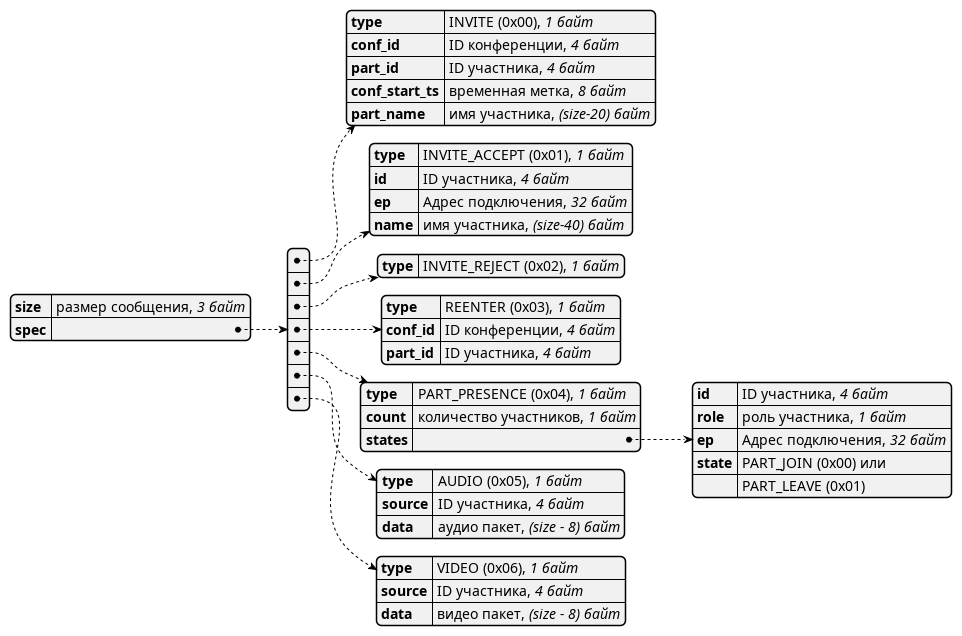
\includegraphics[width=\linewidth]{inc/diag/msg-types/msg-types.png}
  \caption{Схема типов сообщений с полями}
  \label{img:msg-types}
\end{figure}

\section{Медиа форматы}

Снижение объемов передачи аудио/видео данных по сети требует использования кодеков, сжимающих медиа данные. Для разрабатываемого протокола применяются кодеки AAC \cite{aac} и H.264 \cite{h264}. Аудио кадр кодируется в стерео формате с частотой 48кГц. Видео кадр кодируется в разрешении 320 на 180 пикселей и частотой в 30 кадров в секунду.

\section{Взаимодействия сторон}

Рассмотрим сценарий с двумя участниками --- <<А>> и <<Б>>. Для организации конференции, участник <<А>> отправляет участнику <<Б>> сообщение типа \texttt{INVITE}.
После чего участник <<Б>> должен ответить на него сообщением \texttt{INVITE\_ACCEPT} для подключения к конференции участника <<А>>.
После успешного подключения, происходит инициализация каналов передачи медиа данных. Аудио и видео пакеты передаются с использованием сообщений типов \texttt{AUDIO} / \texttt{VIDEO}.
Диаграмма последовательности описанного процесса представлена на рисунке \ref{img:conf-2}.

\begin{figure}[H]
  \centering
  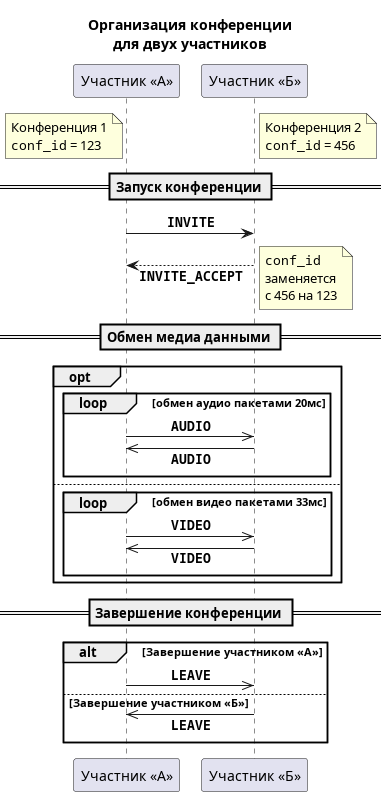
\includegraphics[width=0.6\linewidth]{inc/diag/seq-2/conf-2.png}
  \caption{Диаграмма последовательности для организации конференции для двух участников}
  \label{img:conf-2}
\end{figure}

Подключение последующих участников происходит аналогичным образом --- один из активных участников конференции отправляет сообщение с приглашением в конференцию новому участнику, и, после получения ответного сообщения \texttt{INVITE\_ACCEPT}, отправляет сообщение \texttt{PART\_PRESENCE} остальным участникам конференции для уведомления о подключении нового участника.
Каждый из остальных участников, получив сообщение \texttt{PART\_PRESENCE} отправляет приглашение \texttt{INVITE} новому участнику для инициализации каналов связи между всеми парами участников конференции.
Диаграмма последовательности описанного процесса представлена на рисунке \ref{img:conf-3}.

\begin{figure}[H]
  \centering
  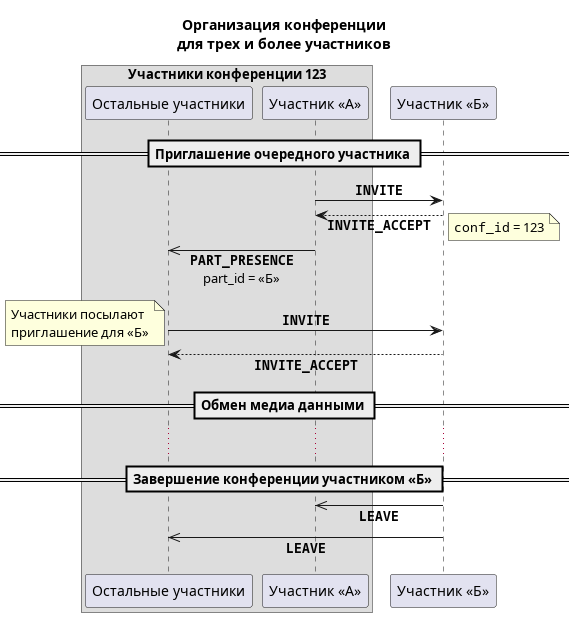
\includegraphics[width=0.9\linewidth]{inc/diag/seq-3/conf-3.png}
  \caption{Диаграмма последовательности для организации конференции для трех и более участников}
  \label{img:conf-3}
\end{figure}

\section{Шифрование}

Шифрование используется для обеспечения целостности и конфиденциальности передаваемых данных. (Защита от подслушивания, порчи и/или подделки сообщений).
Проверка сертификатов разрабатываемым протоколом не предусмотрена, но может быть проведена при повторном соединении с участником.
В качестве протокола шифрования используется TLS v1.3 \cite{tls}.

% TODO: Обоснованность использования TCP вместо RTC и UDP --- TLS не работает поверх UDP?

Выбор между протоколами TCP+TLS и SRTP для организации бессерверных видео конференций зависит от ряда факторов и требований. Рассмотрим преимущества и недостатки каждого из подходов:

Преимущества использования TCP+TLS:

\begin{itemize}[label=---]
  \item Надежность и безопасность --- TCP обеспечивает надежную доставку данных, а TLS предоставляет шифрование и аутентификацию, защищая передаваемые данные.
  \item Совместимость --- TCP и TLS являются широко распространенными и поддерживаемыми протоколами, что упрощает интеграцию с различными системами и платформами.
  \item Развитая инфраструктура --- для TCP+TLS существует большое количество инструментов, библиотек и готовых решений, упрощающих разработку.
  %\item Поддержка NAT и фаерволов --- TCP способен работать через NAT-устройства и фаерволы, что важно для организации бессерверных конференций.
\end{itemize}

Недостатки:

\begin{itemize}[label=---]
  \item Более высокая задержка --- TCP имеет больше накладных расходов по сравнению с UDP-протоколами, что может повлиять на качество аудио и видео.
  \item Более высокие требования к ресурсам --- TCP-стек требует больше памяти и вычислительных ресурсов, что может быть критично для устройств с ограниченными возможностями.
\end{itemize}

Преимущества использования SRTP:

\begin{itemize}[label=---]
  \item Низкая задержка --- SRTP, построенный поверх UDP, имеет меньше накладных расходов, что позволяет обеспечить более высокое качество аудио и видео.
  \item Меньшее потребление ресурсов --- SRTP более эффективен в плане использования памяти и вычислительной мощности, что важно для мобильных устройств.
  \item Специализация на мультимедиа --- SRTP разработан специально для защищенной передачи аудио и видео данных, в отличие от более универсального TCP+TLS.
\end{itemize}
  
Недостатки:

\begin{itemize}[label=---]
  \item Ограниченная совместимость --- SRTP не так широко распространен, как TCP+TLS, что может усложнить интеграцию с существующими системами.
  \item Меньшая надежность --- UDP, лежащий в основе SRTP, не гарантирует доставку данных, что может привести к потере пакетов в неблагоприятных сетевых условиях.
  \item Сложность реализации --- SRTP требует реализации дополнительных механизмов для управления ключами шифрования, что усложняет разработку.
\end{itemize}

%В итоге, выбор между TCP+TLS и SRTP зависит от конкретных требований проекта. TCP+TLS лучше подходит для приложений, где важны надежность, безопасность и совместимость, в то время как SRTP более эффективен для передачи мультимедийных данных с низкой задержкой. Важно также учитывать ресурсные ограничения целевых платформ и сложность реализации каждого из подходов.

\section{Переподключение}

При потере соединения без получения сообщения \texttt{LEAVE} небходимо ожидать переподключение участника в течении 30 секунд. Если участник так и не подключился к конференции, то он считается вышедшим из конференции и в последующем сможет подключиться к ней только через приглашение от другого участника конференции.

Переподключение производится отправкой сообщения \texttt{REENTER} с идентификатором текущей конференции и идентификатором участника, потерявшего соединение. Если сообщение было получено по истечению 30 секундного интервала --- оно отбрасывается, соединение закрывается и участник считывается неподключившимся.

\section{Определение качества каналов связи}

Для реформирования топологии связей в бессерверных видео конференциях необходимо определить качество существующих каналов связи между участниками. Это может быть выполнено с использованием метрик, которые зависят от следующих параметров: временные метки отправки/приема аудио/видео пакета; размер пакета в байтах; количество переданных и повторно переданных пакетов.

На основе этих параметров могут быть вычислены такие показатели качества как:
\begin{itemize}[label=---]
  \item задержка передачи --- временная разница между отправкой и получением пакета;
  \item джиттер --- вариация задержки между последовательными пакетами;
  \item пропускная способность --- объем данных, переданных за определенный период времени.
\end{itemize}

Используя данные метрики, можно оценить состояние каналов связи между участниками конференции и принять решение о необходимости реформирования топологии. Например, если канал между двумя участниками характеризуется высокой задержкой и потерями пакетов, можно рассмотреть вариант передачи медиа данных через третьего участника, который имеет более качественное соединение. Это позволит сократить нагрузку на перегруженный канал и переложить часть вычислительной нагрузки по перекодированию на более мощный клиент.

\chapter{Технологический раздел}

\section{Средства разработки}

Для реализации поддерживающего спроектированный протокол ПО был выбран язык С.
В качестве средства сборки используется средство сборки CMake \cite{cmake}.

Для работы с медиа данными используется библиотека с открытым исходным кодом \texttt{ffmpeg} \cite{ffmpeg}.

Шифрование сообщений осуществляется с использованием библиотеки \texttt{OpenSSL}.

Для автотестов используется фреймворк \texttt{GoogleTest} \cite{gtest}.

\section{Листинги процедуры приглашения}

\includelisting
  {invite-clnt}
  {Процедура приглашения со стороны приглашающего}

\includelisting
  {invite-srv}
  {Процедура приглашения со стороны приглашаемого}

\includelisting
  {invite-worker}
  {Воркер, обрабатывающий входящие приглашения в конференции}

\includelisting
  {invite}
  {Процедура приглашения участника в конференцию}

\section{Сборка и запуск}

Сборка основного проекта осуществляется с использованием утилиты cmake:

\begin{verbatim}
  mkdir build
  cd build
  cmake ..
  make цель
\end{verbatim}
где \textit{<<цель>>} может быть \texttt{selecon\_cli} для сборки консольной утилиты, либо \texttt{unittests} для сборки тестов.

Консольная утилита имеет следующие параметры запуска:

\begin{verbatim}
$ ./selecon_cli --help
./selecon_cli [OPTIONS]

  example demo application for selecon protocol

OPTIONS:
  -h|--help              show this message
  -l|--listen-on address current participant address (default 0.0.0.0:11235)
  -u|--user username     set user name
  --version              print version and exit
  --stub filename        stream given media file in a loop

DESCRIPTION:
  Address can be IPv4/IPv6 (eg: 192.168.100.1:11235) or socket file path
  in format file://<os-path-to-socket>.
\end{verbatim}

Список команд, поддерживаемых утилитой:

\begin{verbatim}
$ ./selecon_cli
> help
list of available commands:
  dev     manage IO devices
  dump    print info about current selecon context state
  exit    end active conference and close cli tool
  help    show this message
  invite  send invitation for joining active conference to other client
  leave   exit conference without exiting cli tool
  quit    same as exit
  say     send text message to conference chat
  sleep   sleep
  stub    set stub media file for playing in conference
\end{verbatim}

В качестве видео заглушки можно использовать видео файлы в формате MP4.

\clearpage

\section{Тестирование ПО}

Ниже приведен список автотестов, разработанных для проверки реализованного протокола. 

\begin{itemize}[label=---]
  \item Подключение второго участника к конференции, второй участник отклонил приглашение.
  \item Подключение второго участника к конференции, второй участник принял приглашение.
  \item Отправка аудио данных от одного участника другому.
  \item Отправка видео данных от одного участника другому.
  \item Подключение четырех участников к конференции.
  \item Отправка аудио данных от одного участника к другим трем.
  \item Отправка видео данных от одного участника к другим трем.
\end{itemize}

\section{Трасировка пакетов}

На рисунке \ref{img:trace-conf-2} представлен сниф пакетов с использованием программы wireshark \cite{wireshark} во время инициализации конференции с двумя участниками.
На рисунке \ref{img:trace-conf-2-tls} представлен сниф того же сценария, но с использованием TLS протокола.

\begin{figure}[h!]
  \centering
  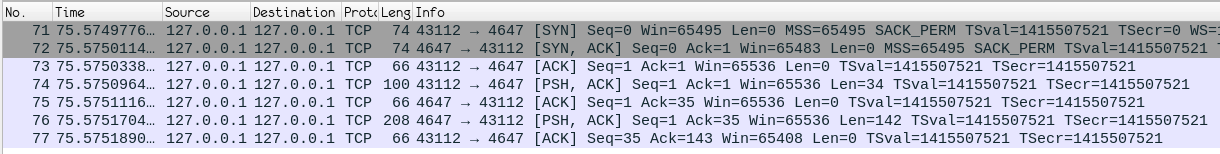
\includegraphics[width=\linewidth]{inc/img/trace-conf-2.png}
  \caption{Сниф wireshark соединения двух участников без использования TLS}
  \label{img:trace-conf-2}
\end{figure}

\begin{figure}[h!]
  \centering
  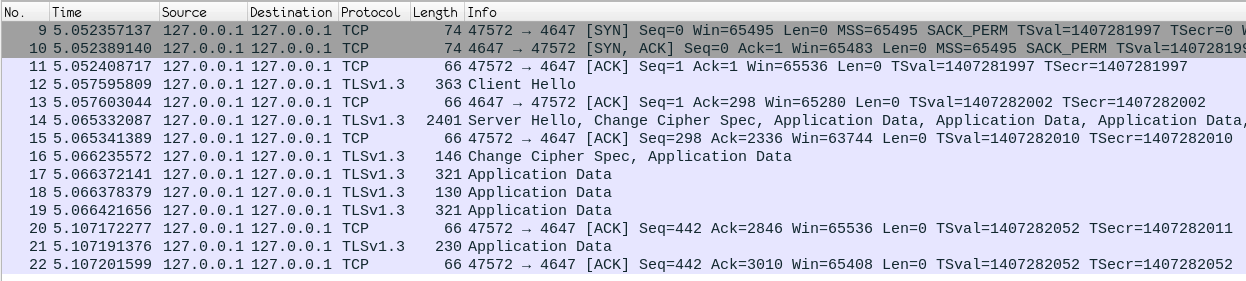
\includegraphics[width=\linewidth]{inc/img/trace-conf-2-tls.png}
  \caption{Сниф wireshark соединения двух участников с использованием TLS}
  \label{img:trace-conf-2-tls}
\end{figure}

\clearpage

На рисунках \ref{img:trace-conf-3}--\ref{img:trace-conf-3-tls} представлены снифы пакетов во время инициализации конференции с тремя участниками. По рисунку видны 3 этапа соединения: инициализация конференции двумя участниками; отправка и получение приглашения для третьего участника и информирование второго участника о новом подключившемся участнике; рукопожатие второго и третьего участников.

\begin{figure}[h!]
  \centering
  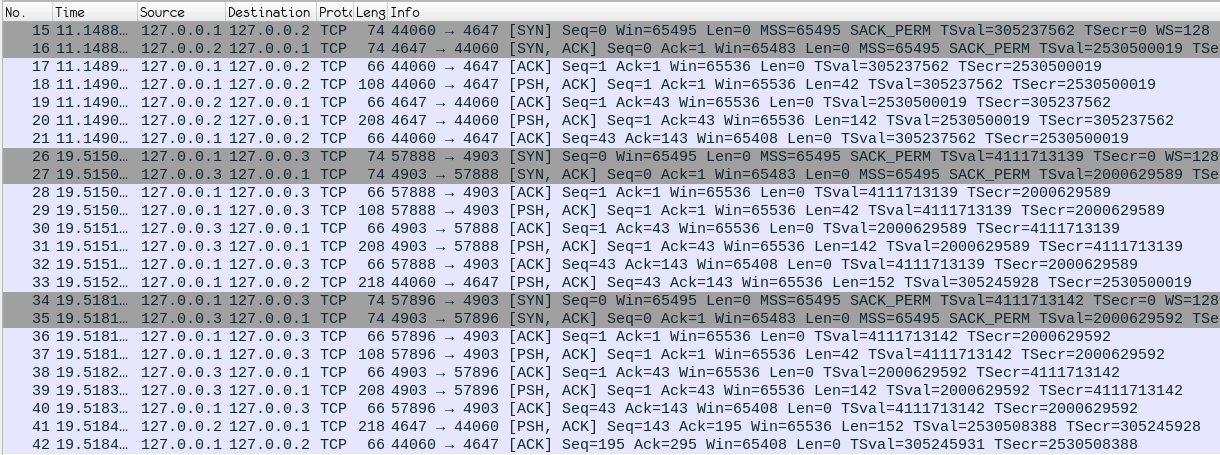
\includegraphics[width=\linewidth]{inc/img/trace-conf-3.png}
  \caption{Сниф wireshark соединения трех участников без использования TLS}
  \label{img:trace-conf-3}
\end{figure}

\begin{figure}[h!]
  \centering
  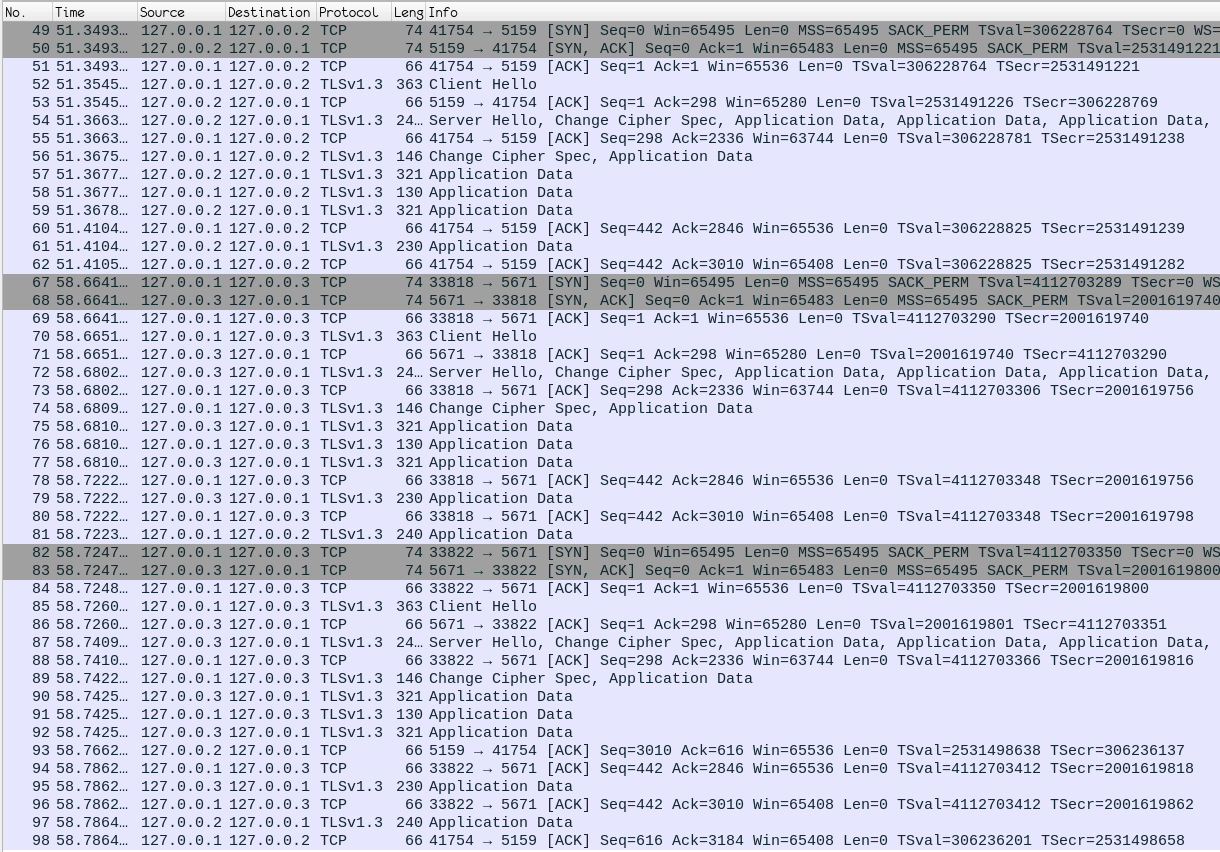
\includegraphics[width=\linewidth]{inc/img/trace-conf-3-tls.png}
  \caption{Сниф wireshark соединения трех участников с использованием TLS}
  \label{img:trace-conf-3-tls}
\end{figure}

\chapter{Исследовательский раздел}

\section{Постановка исследования}

Цель исследования --- выявление зависимости задержки аудио и видео, а также общей нагрузки на процессор от числа участников в конференции.

Исследование проведено на ноутбуке Intel i5-8365U 4.1GHz, 16GB оперативной памяти, под операционной системой Debian 12.

Количество участников варьируется от 2 до 7, время конференции --- 1 минута. Во время конфереции все участники транслировали одно и то же видео.

\section{Результаты}

Результаты представлены на графике \ref{img:latency}.

\begin{figure}[h!]
  \centering
  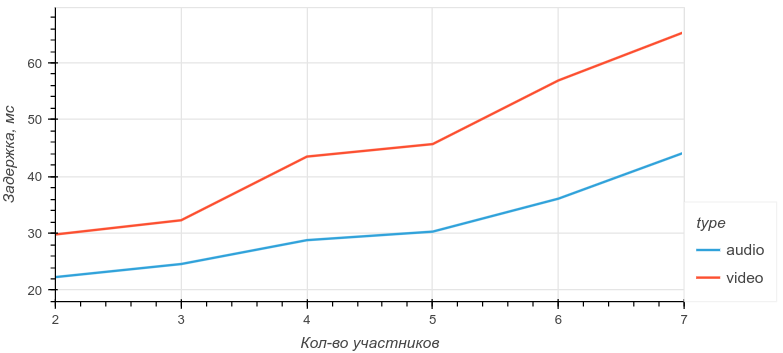
\includegraphics[width=\linewidth]{inc/img/latency.png}
  \caption{Зависимость средней задержки аудио и видео от числа участников конференции}
  \label{img:latency}
\end{figure}

На основе полученных результатов можно предположить, что увеличение задержки связанно с  увеличивающейся нагрузкой на процессор при увеличении количества участников.

% \section*{Выводы}

\chapter*{ЗАКЛЮЧЕНИЕ}
\addcontentsline{toc}{chapter}{ЗАКЛЮЧЕНИЕ}

В результате работы был спроектирован протокол бессерверных конференций. Разработана программная реализация спроектированного протокола и реализовано ПО, осуществляющее пересылку видео и аудио потоков в рамках бессерверной конференции. Проведено тестирование и исследование ПО. В результате исследования была выявлена зависимость задержки видео и аудио потоков от количества участников конференции.


}

\makebibliography

\begin{appendices}
%	\chapter{} % design

	% \includelisting
	% 	{tinygo}
	% 	{Грамматика языка TinyGO}

	% \chapter{} % impl

	%\includelisting
%		{defer}
%		{Реализация алгоритма добавления отложенного вызова}
	
%	\includelisting
%		{multiret}
%		{Реализация обработки определения функций, возвращающей несколько значений}
	
%	\includelisting
%		{makefile}
%		{Скрипт сборки и запуска компилятора}

%	\chapter{} % test

%	\includelisting
%		{test-src}
%		{Исходный код теста --- работа с динамическим списком}

%	\includelisting
%		{test-llvm-out}
%		{Результат преобразования тестового кода в промежуточный код LLVM}

%	\chapter{} % research

%	\includelisting
%		{research-src}
%		{Исходный код для проведения исследования}

\end{appendices}

\end{document}